\documentclass[a4paper,oneside]{book}
\usepackage{caption}
\usepackage{a4wide}
\usepackage{makeidx}
\usepackage{float}
\usepackage{listings}
\usepackage{color}
\usepackage{textcomp}
\usepackage{alltt}
\usepackage{amsmath}
\usepackage{times}
\usepackage{ifpdf}
\usepackage{graphicx}
\usepackage{color} %colors in text
\usepackage{textcomp} % 
\usepackage[T1]{pbsi} %hand writting nice 
\usepackage[T1]{fontenc} %more fonts
\usepackage{mathrsfs} % letters for math
\usepackage{amsmath} % math formulas
\usepackage[all]{xy} % for drawing
\usepackage{listings}
\usepackage{amssymb}
%\usepackage[parfill]{parskip}
\definecolor{gray}{rgb}{0.7,0.7,0.7} 
\usepackage{enumerate} %for enumerate
\usepackage{subfigure}
\usepackage{epsfig}
\usepackage{float}
\usepackage{algorithm}
\usepackage[noend]{algorithmic}
\usepackage[dvipdfm]{hyperref}
\usepackage{multicol}
\usepackage{sectsty}
\usepackage{multirow}
%\ifpdf
%\usepackage[pdftex,
%            pagebackref=true,
%            colorlinks=true,
%            linkcolor=blue,
%            unicode
%           ]{hyperref}
%\else
%\usepackage[ps2pdf,
%            pagebackref=true,
%            colorlinks=true,
%            linkcolor=blue,
%            unicode
%           ]{hyperref}
%\usepackage{pspicture}
%\fi
\usepackage[utf8]{inputenc}
\makeindex
\setcounter{tocdepth}{3}
%\usepackage[light,condensed,math]{kurier}
\renewcommand{\thechapter}{\Roman{chapter}}
%DEFINE NEW COMMANDS_________________________________________________________
\newcommand{\clearemptydoublepage}{%
  \newpage{\pagestyle{empty}\cleardoublepage}%
}
\newcommand{\ds}{\displaystyle}
\newcommand{\todo}[1]{\textcolor{red}{\textbf{#1}}}
\newcommand{\fade}[1]{\textcolor{gray}{\textbf{#1}}}
\newcommand{\myemph}[1]{{\normalfont\emph{#1}}}

\newcommand{\tit}{\textit}

%____________________________________________________________________________
\begin{document}
	%THE TITLE PAGE & STUFF_________________________________________________________________
	%\fontfamily{arial}\selectfont
	%\fontfamily{courier-ttf}\selectfont
	%\fontfamily{comicsans}\selectfont
	%\fontfamily{franklingothic}\selectfont
	%\fontfamily{impact}\selectfont Impact
	%\fontfamily{palatino-ttf}\selectfont
	%\fontfamily{sylfaen}\selectfont 
	%\fontfamily{tahoma}\selectfont
	%\fontfamily{times-ttf}\selectfont 
	%\fontfamily{trebuchet}\selectfont 
	%\fontfamily{verdana}\selectfont 
	\fontfamily{georgia}\selectfont\normalsize

	\hypersetup{pageanchor=false}
	\begin{titlepage}
	\begin{figure}[!hbtp]
		\begin{flushright}
			
\epsfig{file=images/uva.eps, width=0.3\linewidth}
		\end{flushright}
	\end{figure}
	\vspace*{2cm}
	\begin{center}
	\rule{\linewidth}{1px}\\[10pt]
	\Huge{Texture Synthesis for Material Classification}
	\rule{\linewidth}{1px}\\[10pt]
	\vspace*{1cm}
	\large{Master\rq s Thesis in Artificial Intelligence -- Intelligent Systems}
	\large
	\vspace*{4cm}
	\begin{multicols}{2}
		\begin{flushleft}
			{\emph{Author:}\\
			Jasper van Turnhout\\
			\textit{jturnhou@science.uva.nl}\\ 
			Student number: 0312649}  
		\end{flushleft}
		\begin{flushleft}
			{\emph{Supervisors:}\\
			\href{mailto:Th.Gevers@uva.nl}{Prof. dr. Theo Gevers}\\
			\href{mailto:geusebroekuva.nl}{Dr. Jan-Mark Geusebroek}\\
			Informatics Institute, Faculty of Science, University of Amsterdam\\
			}
		\end{flushleft}
	\end{multicols}
	\end{center}
	\vspace*{6cm}
	\end{titlepage}
	%ABSTRACT PAGE____________________________________________________________________________
	\thispagestyle{empty}
	\section*{Abstract}
		Research description comes here
	%CONTENT PAGE____________________________________________________________________________
	\newpage
	\pagenumbering{roman}
	\tableofcontents
	%CHAPTERS & SUB-CHAPTERS____________________________________________________________________
	\newpage
	\pagenumbering{arabic}
	\hypersetup{pageanchor=true}
	\chapter{Introduction}
	\hypertarget{Introduction}{
}

For human perception, recognizing materials is a very important aspect in our visual system. We can do this flawlessly for a great number of different materials. As a human, we can easily determine whether a surface is smooth, rough, soft or hard by just looking at it. We are also capable of recognizing  materials under great variety of visual conditions. For example, when observing a car from an arbitrary point of view, we always perceive the surface of the car differently when considering the light reflected on the metallic surface which differs from viewpoint to viewpoint. Yet, we have no problem in classifying this surface as metal. The same accounts for many other materials we perceive on a daily base.

Material recognition is a field of research in computer vision with the goal to develop classification systems that can identify various material categories observed in daily life. Examples of such categories are metal, wood, fabric, plastic and glass. Material recognition differs and should not be confused with object recognition and texture recognition. This difference is illustrated in figure \ref{fig:ObjectRecognition} and \ref{fig:TextureRecognition}. A system capable of recognizing materials can greatly enhance the performance of object recognition or scene recognition.

Research has been done on several different material databases and good recognition accuracies have been reported. However, there are suggestions that the accuracies reported are all database dependent \cite{ExploringFeatures} since none of these databases could possibly capture the large variation in appearance of material classes. The large variation of a material class is also addressed as the intra-class variation. 

In this research, we investigate how realistic image synthesis can be employed to create synthetic image data for various material classes. With the aid of image synthesis it is possible to generate infinite amounts of data with arbitrary viewpoint and illumination conditions. This makes it possible to create image data that is not present in material databases, thus making it possible to increase the intra-class variation of material classes.

This chapter gives a short introduction to the problem of material recognition and how image synthesis can be applied to improve recognition performance.

\begin{figure}[htbp!]
	\begin{center}
		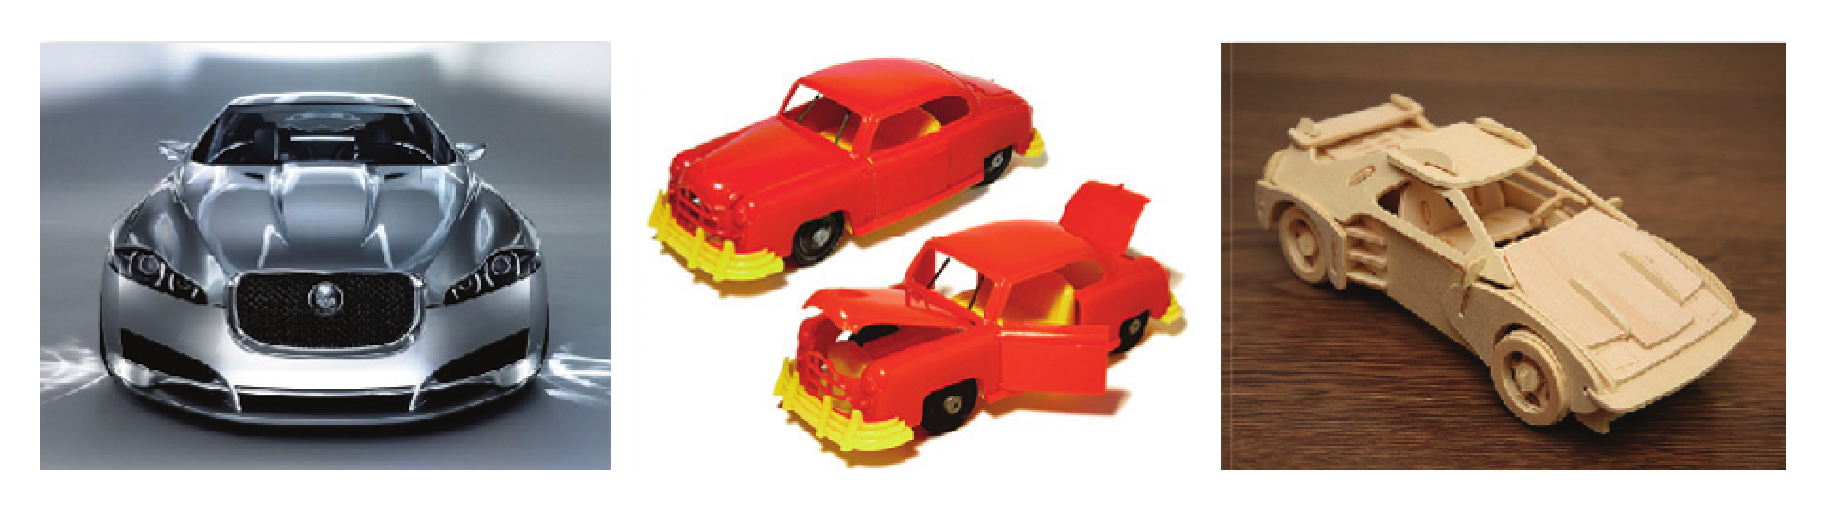
\epsfig{file=images/ObjectRecognition.eps, width=0.6\linewidth}
	\end{center}
	\caption{{\it Object recognition and material recognition: all three pictures depict the same object. However, they are made from metal, plastic and wood respectively. Image adapted from \cite{ExploringFeatures}.}}
	\label{fig:ObjectRecognition}
\end{figure}

\begin{figure}[htbp!]
	\begin{center}
		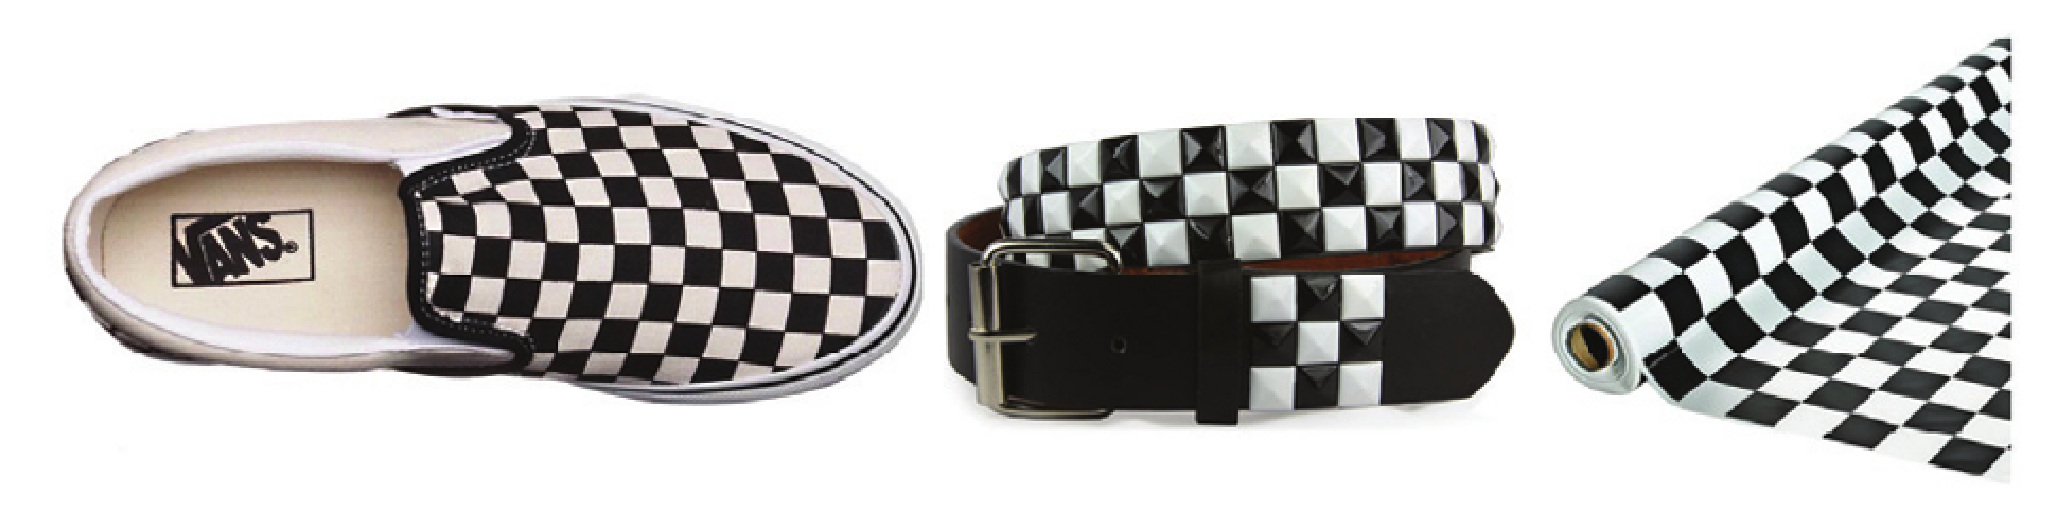
\epsfig{file=images/TextureRecognition.eps, width=0.6\linewidth}
	\end{center}
	\caption{{\it Texture recognition and material recognition: all three pictures depict the same pattern. However, they are made from fabric, plastic and paper respectively. Image adapted from \cite{ExploringFeatures}.}}
	\label{fig:TextureRecognition}
\end{figure}

\section{Material Recognition}
Material recognition is defined as the task to correctly classify a novel image from a material surface. When building a system for material recognition, prediction of a material class is done preferably on a single image of a material surface. This creates a difficult task as the variation in appearances of materials is considerably enhanced by illumination differences or arbitrary viewpoints. Some examples of how much a surface can vary are shown in figure \ref{fig:PhoTexExamples}.

In recent research, material databases have been created containing various illumination and viewpoint conditions that try to capture the large variety within each  material class. The difficulty is to obtain robust features from the image data that covers various occurrences of materials with different spatial properties as well as distinct illumination properties. 

\begin{figure}[htbp!]
	\begin{center}
		\subfigure[aab]{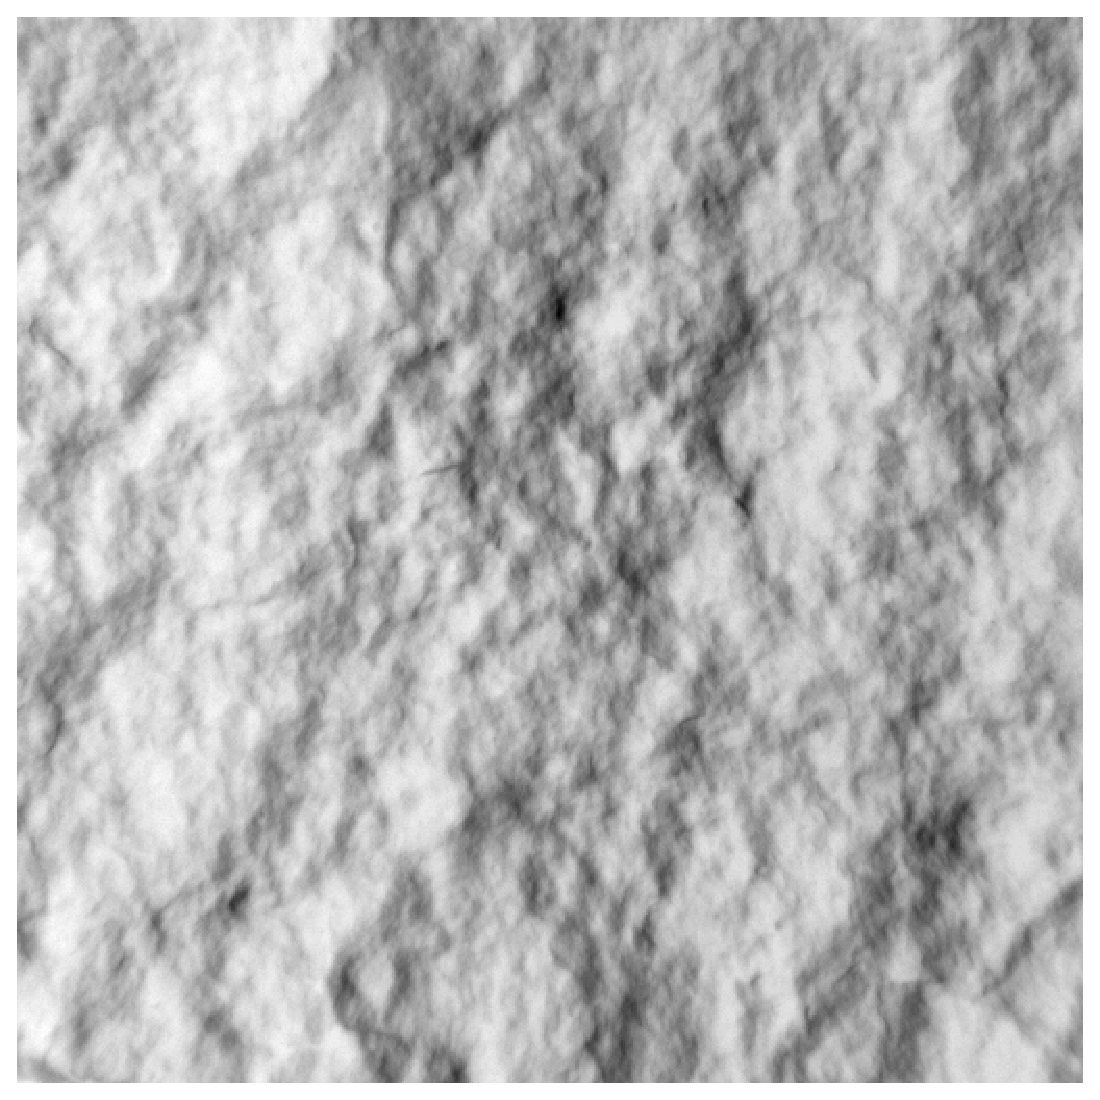
\epsfig{file=images/examples/0.aab.0.30.0.eps, width=0.15\linewidth}}\label{fig:aab1}
		\subfigure[acd]{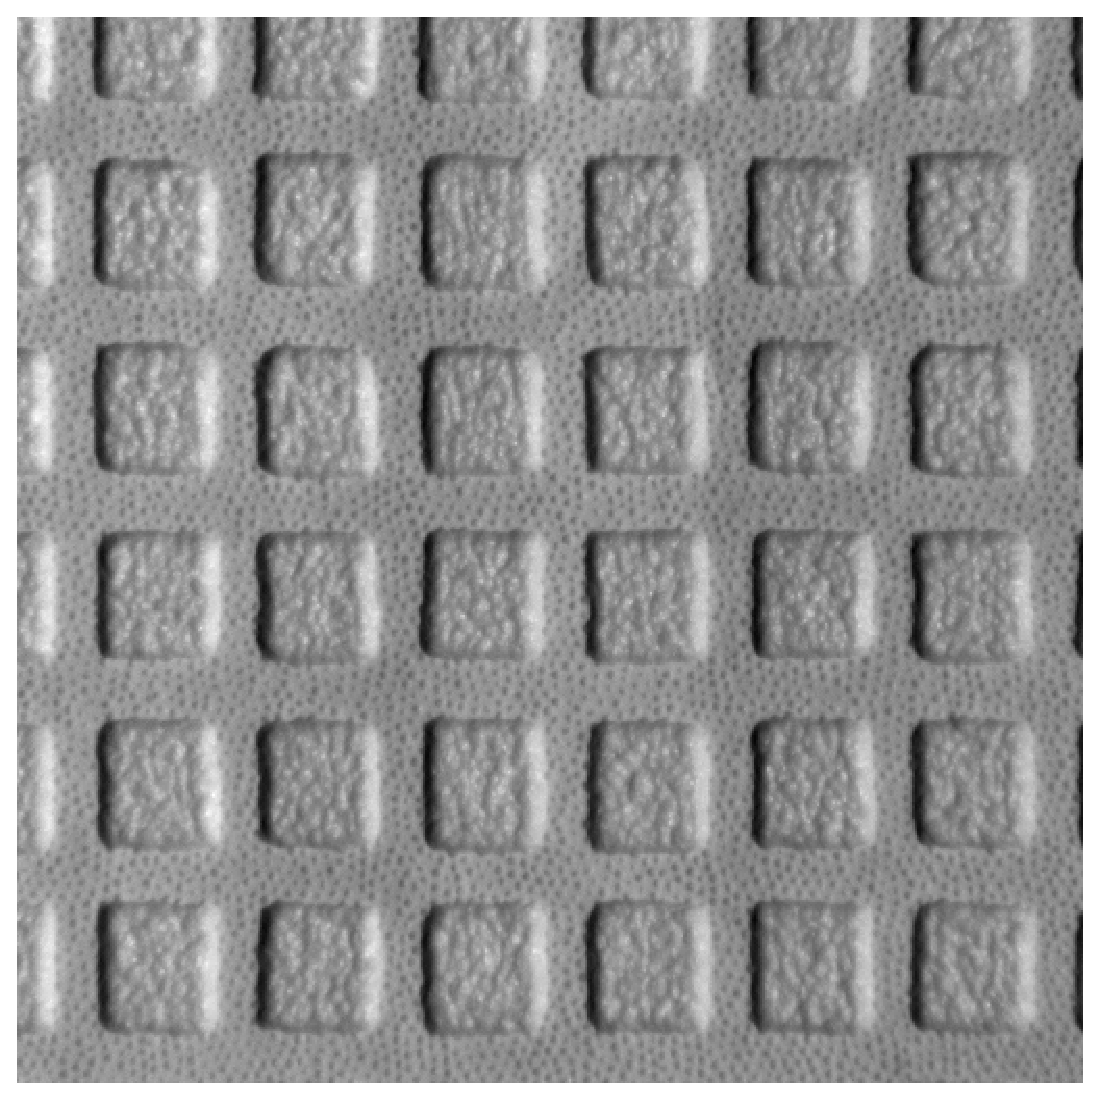
\epsfig{file=images/examples/1.acd.0.30.0.eps, width=0.15\linewidth}}\label{fig:acd1}
		\subfigure[adh]{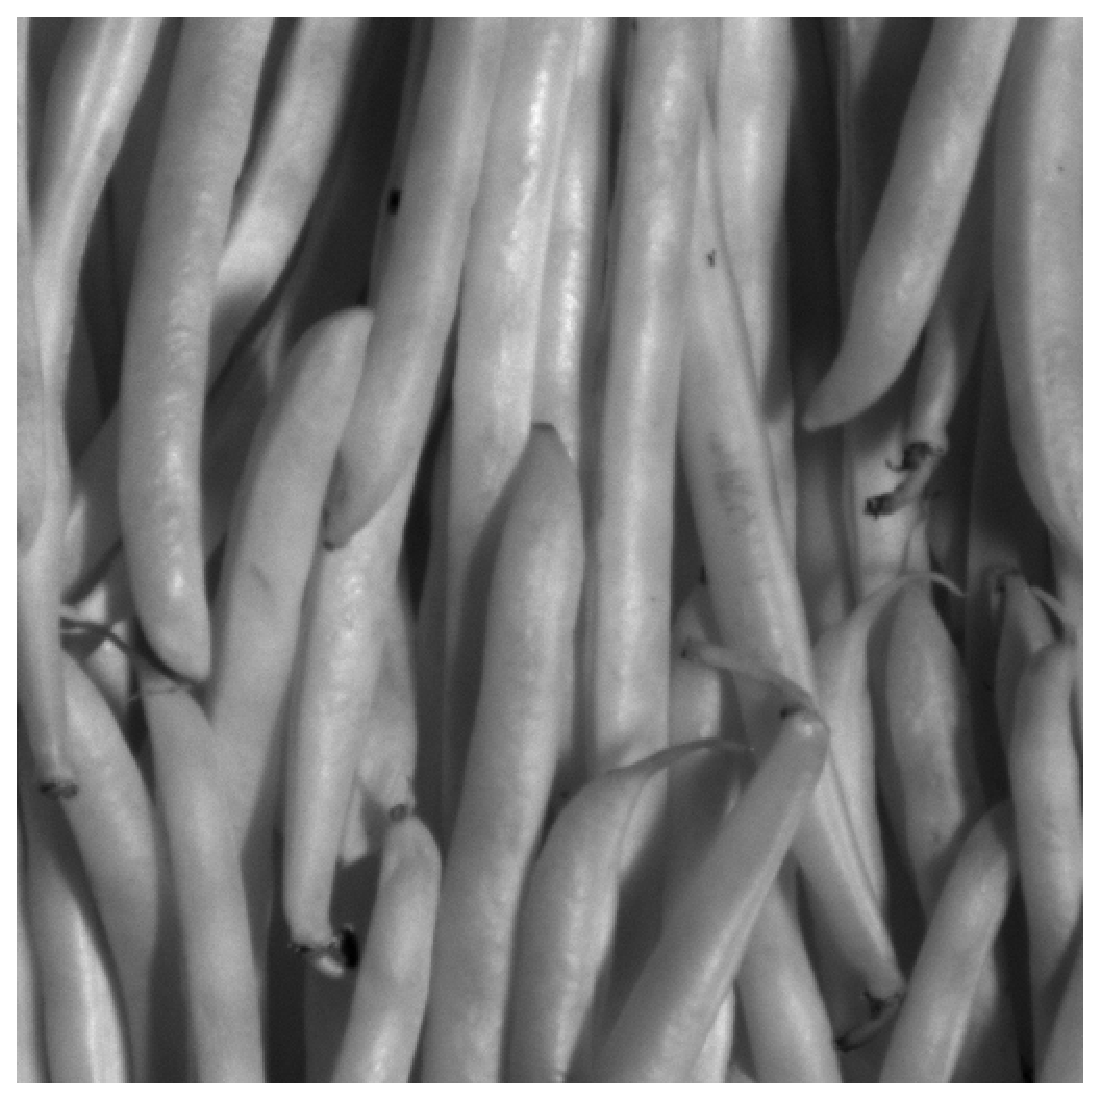
\epsfig{file=images/examples/2.adh.0.30.0.eps, width=0.15\linewidth}}\label{fig:adh1}

		\subfigure[aab]{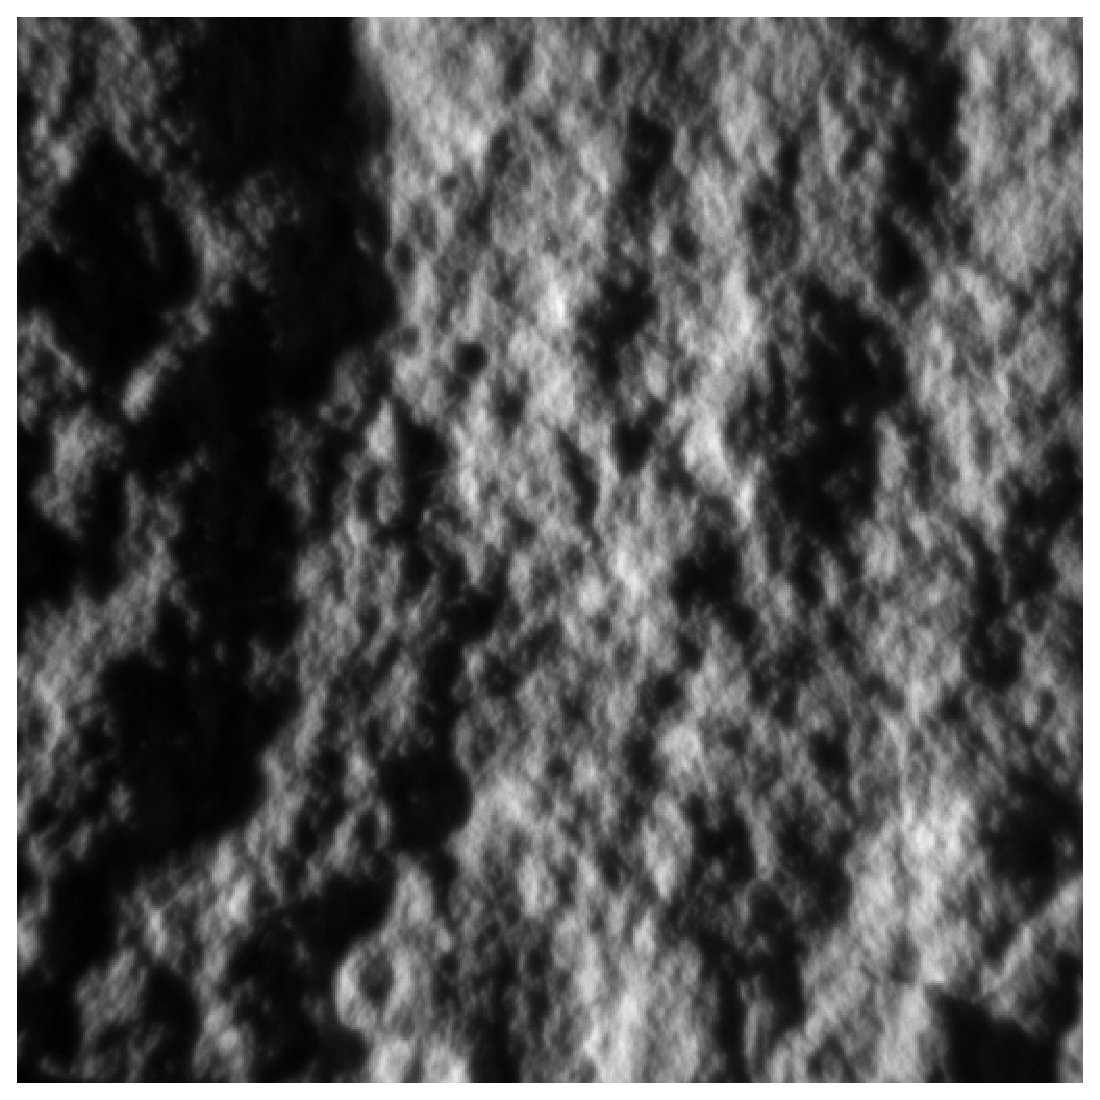
\epsfig{file=images/examples/0.aab.0.75.180.eps, width=0.15\linewidth}}\label{fig:aab2}
		\subfigure[acd]{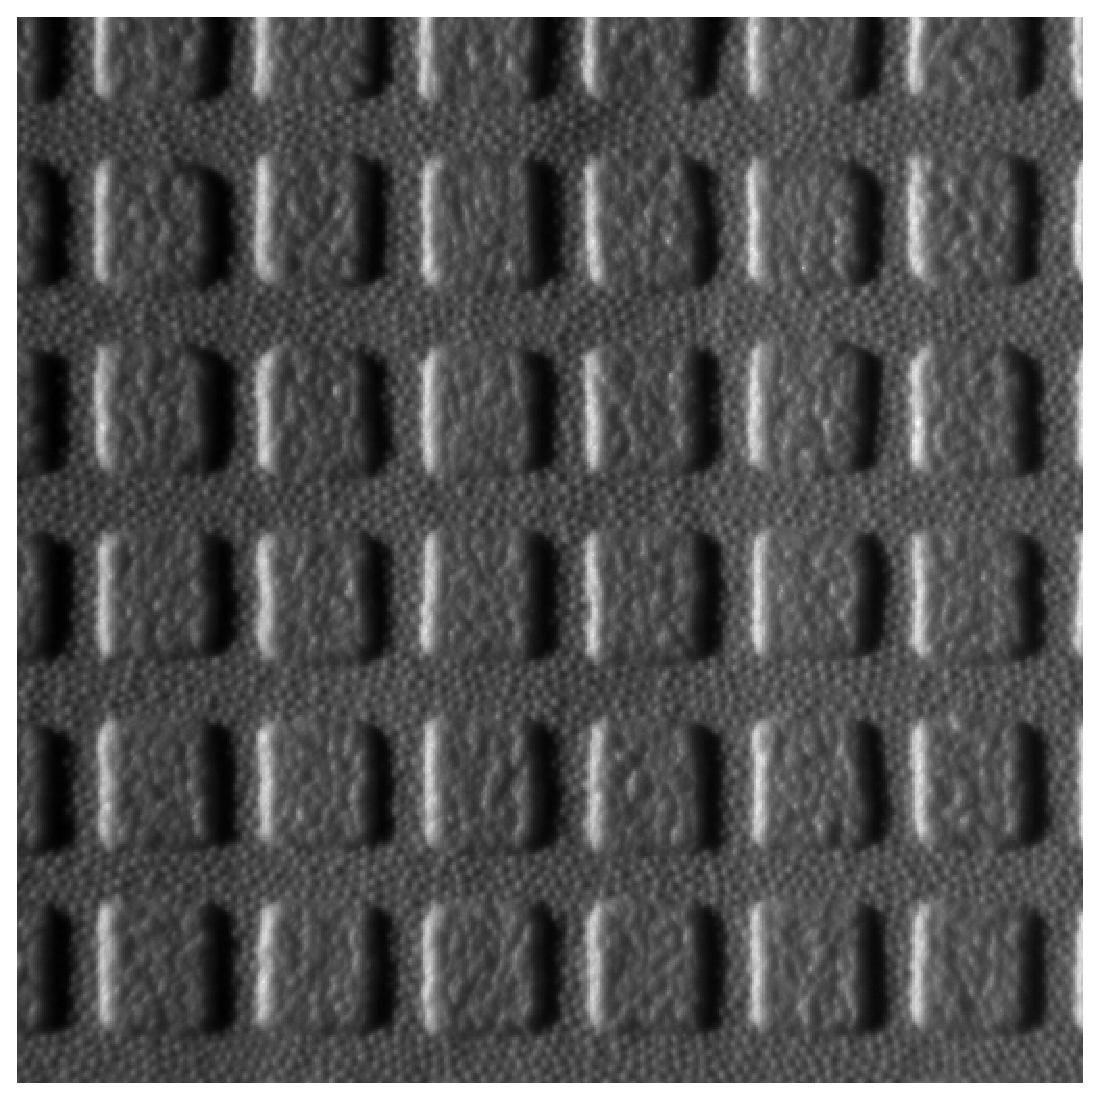
\epsfig{file=images/examples/1.acd.0.75.180.eps, width=0.15\linewidth}}\label{fig:acd2}
		\subfigure[adh]{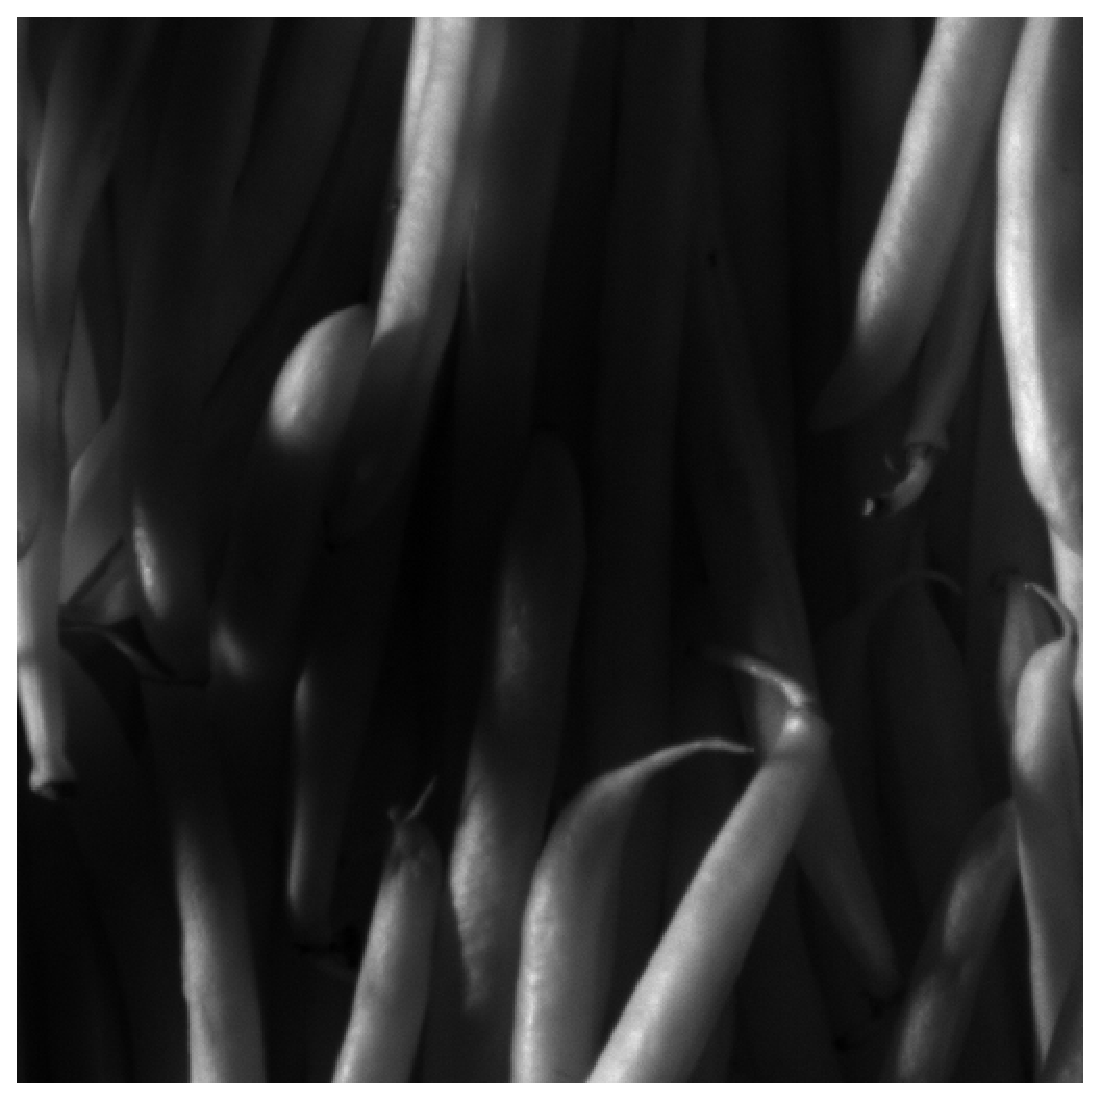
\epsfig{file=images/examples/2.adh.0.75.180.eps, width=0.15\linewidth}}\label{fig:adh2}
	\end{center}
	\caption{{\it Example images from the PhoTex database. The upper row is recorded under a slant of $30^0$ and a tilt of $0^o$. The lower row is recorded under a slant of $75^0$ and a tilt of $180^0$. The captions are the material labels.}}
	\label{fig:PhoTexExamples}
\end{figure}

The {\it CuRET} database captures such properties for 60 different material classes with each over 200 different illumination and viewing directions. This database has been used in the development of texton descriptors to capture the various material properties. In later research on the {\it CuRET} database, parametric models have been developed to deal with the limits of a texton dictionary. The {\it ALOT} and {\it PhoTex} databases have been used in more physically-based computer vision experiments where the geometrical structure of the surface is used for development of robust descriptors. In all these experiments, classification rates of 95\% and higher are reported using various methods such as Naive Bayes, Nearest Neighbor and Support Vector Machines.

The reported classification rates are of great accuracies in general, it seems that most of the difficulties have been solved for material recognition. However, the suggestion that the databases do not capture the intra-class variety for the material classes poses the problem of data shortage. Recording the data is a time-consuming task and will not be sufficiently diverse to capture all possible illumination and viewing directions. 

\section{Image Synthesis}
The field of computer graphics has accomplished imagery of great realism over the past few decades. With increasing computational power, it became possible to synthesize realistic images using expensive physically-based light simulations. 

Various models have been developed for the synthesis of diffuse, glossy or shiny materials. These models use as input for per-pixel generation of an image a surface normal, the surface albedo, a viewing direction, an illumination direction and illumination properties such as the color of the light source. With proper reconstruction of the surface normals and surface albedo for a material, it is possible to generate an infinite amount of data with arbitrary viewing and illumination directions. Databases such as {\it PhoTex} and {\it ALOT} were created with physically-based computer vision in mind. With image data available for each material class with recorded light source directions, it is possible to recover surface normals and surface albedo for material classes. 

In research done by Targhi \cite{Targhi}, the synthesis of material images has been used to augment training-sets to a point of saturation where perfect predictions were made \cite{Targhi}. For the synthesis of image data, the Lambertian reflection model was used. This reflection model is limited to the synthesis of purely diffuse materials only, since the reflection model does not simulate illumination phenomena such as speculars which are observed on glossy and shiny surfaces. Other reflection models should be considered as well if we want to be able to synthesize images for other than purely diffuse materials.

\section{Goal of this thesis}
In this research, the aim is to investigate the addition of more sophisticated reflection models for the synthesis of realistic image data. We research and implement combinations of Lambertian reflectance with models for speculars such as Phong, Blinn-Phong and Torrance-Sparrow, as well as a more sophisticated model for diffuse reflection. 

The synthetic image data is used for training models for material classification. These models are tested against two datasets: a dataset consisting of mainly diffuse materials and a dataset consisting of shiny/glossy materials. Our main focus is to test and compare performance of classification when using only synthetic image data for training the models for classification. With the addition of specular reflection models for synthesis, we can expect some improved models when comparing the performance with models obtained from synthetic data using Lambertian reflection only.

\section{Overview of this thesis}
In the next chapter, some of the state-of-the-art methods and their experiments are outlined. Some of these methods are adapted for the experiments in this research. In chapter 3, the methods that we adapt in this research will be discussed in more detail. Chapter 4 outlines some fundamentals that are used for understanding the reflection models. In chapter 5, a set of empirical reflection models that we implemented for the experiments are discussed in detail. In chapter 6, a set of more physical-based reflection models that we implemented are discussed in detail. In chapter 7, the experiments and their results are reported and the last chapter holds the conclusion and future works.


	\chapter{Related work}
	\hypertarget{RelatedWork}{
}
In earlier research on the topic of material recognition, the main focus was on the albedo variation on top of a flat surface. More recently, this focus has shifted towards surface normals, which cause the $3\mathcal{D}$ effects we perceive in the $2\mathcal{D}$ through shadows and speculars. In this section, three state-of-the-art methods are outlined.

The first method --- presented in section \ref{sec:Textons} --- relies on the construction of a texton dictionary which is afterwards used for feature extraction. The second --- described in section \ref{sec:MGD} --- computes a marginal distribution out of the 8 maximum responses of the convolution of each image with a fixed set of filters. Finally, in section \ref{sec:Minimal} a novel idea is presented in which the performance of a material recognition system is enhances by adding synthetic image data.


\section{Textons}\label{sec:Textons}

The need for larger material databases that capture the variety in viewpoint and illumination resulted in the creation of the {\it CUReT} database. Dana and Nayar \cite{DanaNayar} developed parametric models \todo{based on surface roughness and correlation lengths} which were tested against the {\it CUReT} database. However, in their research, no significant results were reported \cite{VarmaZisserman}.

Leung and Malik were the first to introduce the texton modeling method to the problem of illumination variation \cite{LeungMalik}. In their research, they introduce the concept of 2 and 3-dimensional textons based on Gaussian derivative filters. These Gaussian filters capture certain properties of a material on microscale; for example, a point $n(x,y)$ in an image of a material can correspond to a ridge, bump, groove, spot, etc. A filter-bank of different Gaussian filters can capture these properties in the response of the image applied to such filter. This makes it able to capture the variance of materials under different illuminations using a representable set of filters.

\begin{figure}[b]
	\begin{center}
		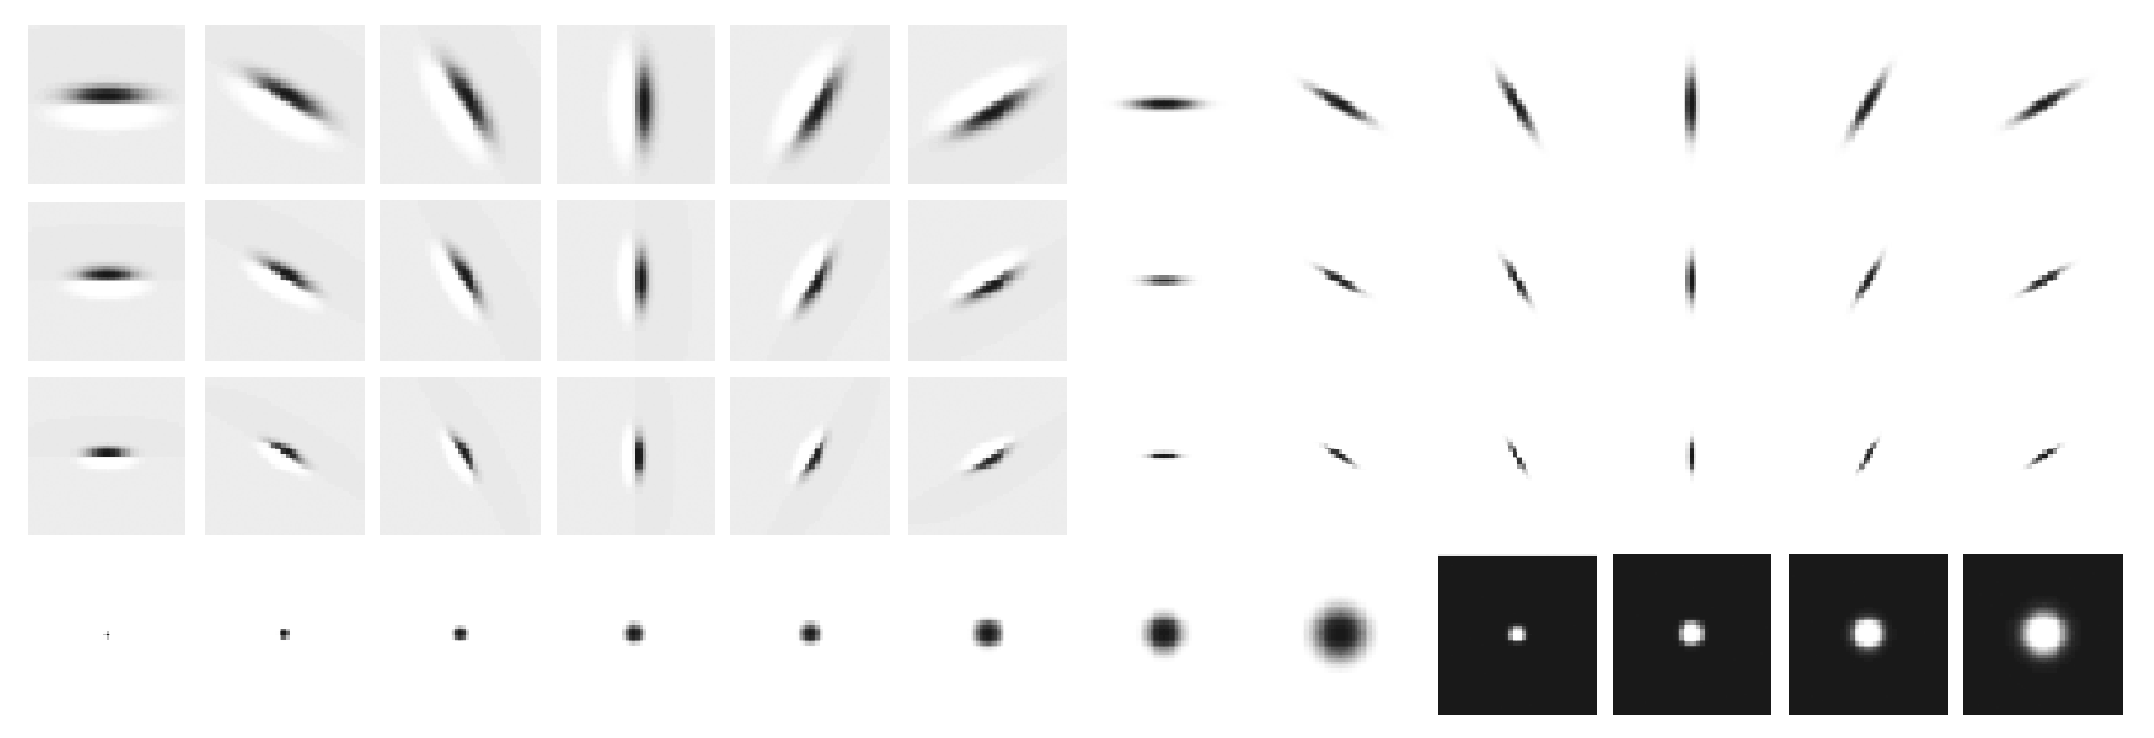
\epsfig{file=images/LM.eps, width=0.6\linewidth}
	\end{center}
	\caption{\textit{LM filter bank, consisting of an edge, bar and spot filter at multiple orientations and scales. 2 Gaussian derivatives at 6 orientations and 3 scales, 8 Laplacian of Gaussian filters and 4 Gaussian filters give a total of 48 filters in the filter bank.}}
	\label{fig:LM}
\end{figure}


In the case of a $2\mathcal{D}$ texton, a material is characterized by responses obtained by convolving images from this material with a set of orientation- and spatial-frequency linear filters. As a result, every pixel in an image is now represented as a vector of $N_{fil}$ corresponding response values, where $N_{fil}$ is the number of filters in the filter bank. With the obtained set of vectors of size $N_{fil}$, they use a K-means algorithm to find a number of vectors as representable clusters in this vector space. The clusters found by K-means give the $2\mathcal{D}$ texton descriptors. These texton descriptors represent characteristics such as ridges, bumps, etc. of the material under a given illumination.

Because a material under a different illumination can appear completely changed due to effects of masking, shadowing, specularity or global illumination, a $2\mathcal{D}$ texton is not enough to capture the general characteristics of a material. As already shown in figure \ref{fig:PhoTexExamples}, the appearance of a material appearances change drastically under different illumination conditions. A great amount of shadows and masking effects make it hard to classify image \ref{fig:PhoTexExamples}(f) when the textons are computed from image \ref{fig:PhoTexExamples}(c), since these effects are not properly quantized by the textons. 

To capture such effects, many images with different illumination variation and viewing directions from the same material are needed. Given a number of images $N_{img} \gg 1$,  concatenating the responses of these $N_{img}$ images will give high dimensional $N_{fil}N_{img}$ data vectors. Clustering these data vectors with K-means will give cluster centers which encode the dominant properties in all the images belonging to a certain material class. These cluster centers represent the $3\mathcal{D}$ textons and encode various image properties like illumination changes, spatial properties (bumps, ridges, etc.), as well as reflectance properties of the material (shiny/glossy as well as diffuse properties). Given the wide range of material characteristics captured by the $3\mathcal{D}$ textons, they represent strong descriptors for the problem of illumination variation within material recognition.

The set of $3\mathcal{D}$ textons --- K-means cluster centers --- over all classes will serve as a texton dictionary for the construction of histograms. Using the same responses as before, for a training image, a histogram is constructed by assigning every vector corresponding to a pixel in the image to a texton in the dictionary using the $\chi^2$ (Chi Square) statistic to measure distance between vector and textons. The histogram is a representation of the image in terms of features, as encoded in the texton dictionary. With this quantization procedure, each material class can be represented by a set of histograms. To classify a novel image, responses are computed, a histogram is constructed using the texton dictionary, and a Nearest Neighbor algorithm is employed to find the histogram in the training set that is closest to it. The function used to measure distances between histograms is again $\chi^2$.

Originally, Leung and Malik used a set of 48 Gaussian derivative filters to compute the responses on an image. Varma and Zisserman extended this research by observing the effect of various filter banks for the computation of the responses \cite{VarmaZisserman}. In their experiments, using a similar setup to that of Leung and Malik, they construct texton dictionaries based on different filter banks and compare performance to the filter bank proposed by Leung and Malik. The filter banks used in these experiments were the Schmid (S) set and the Maximum Response (MR) sets. 

The S set consists of 13 isotropic Gabor-like, rotationally invariant filters. The MR sets consist of 38 Gaussian derivative filters: 2 anisotropic filters for edges and bars, on 6 orientations and 3 scales, and 2 isotropic filters, a Gaussian and a Laplacian of a Gaussian filter. They used two version of this set in their experiments. The MR8 set, only the top 8 responses are recorded by taking the maximum response of the anisotropic filters at each scale over all orientations and taking the responses of both isotropic filters. The MR4 set is a subset of the MR8 set, where the anisotropic filters only occur on a single fixed orientation.

The experiments showed a significant difference in performance for the different filter banks. The best classification accuracy is obtained when using the MR8 filter bank.

\begin{figure}[t]
	\begin{center}
		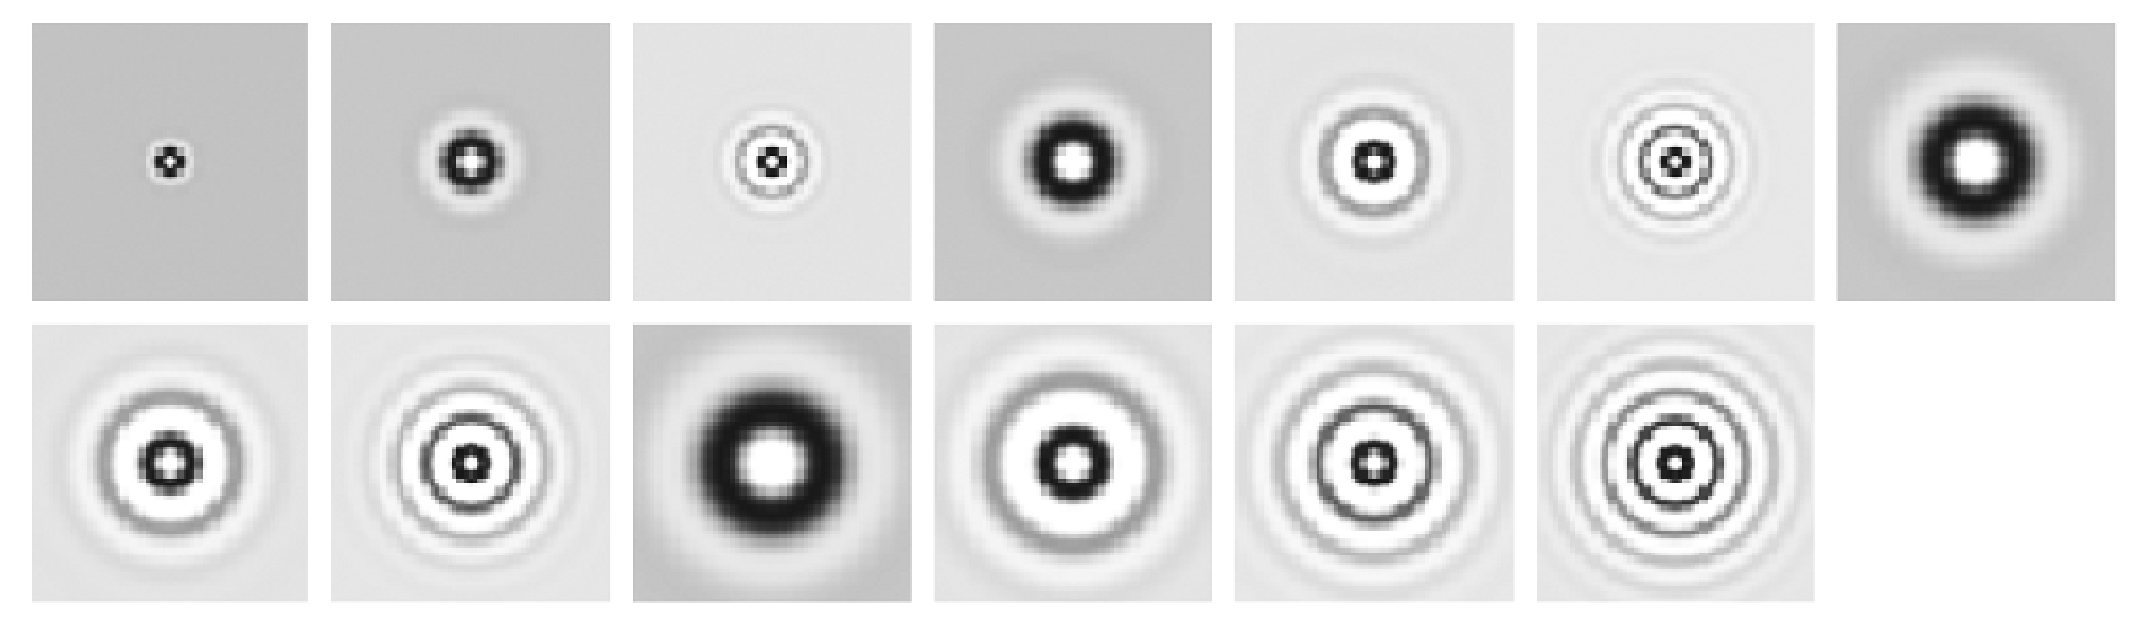
\epsfig{file=images/S.eps, width=0.6\linewidth}
	\end{center}
	\caption{\textit{The Schmid filter bank consists of 13 isotropic rotationally invariant filters.}}
	\label{fig:S}
\end{figure}

\begin{figure}[b]
	\begin{center}
		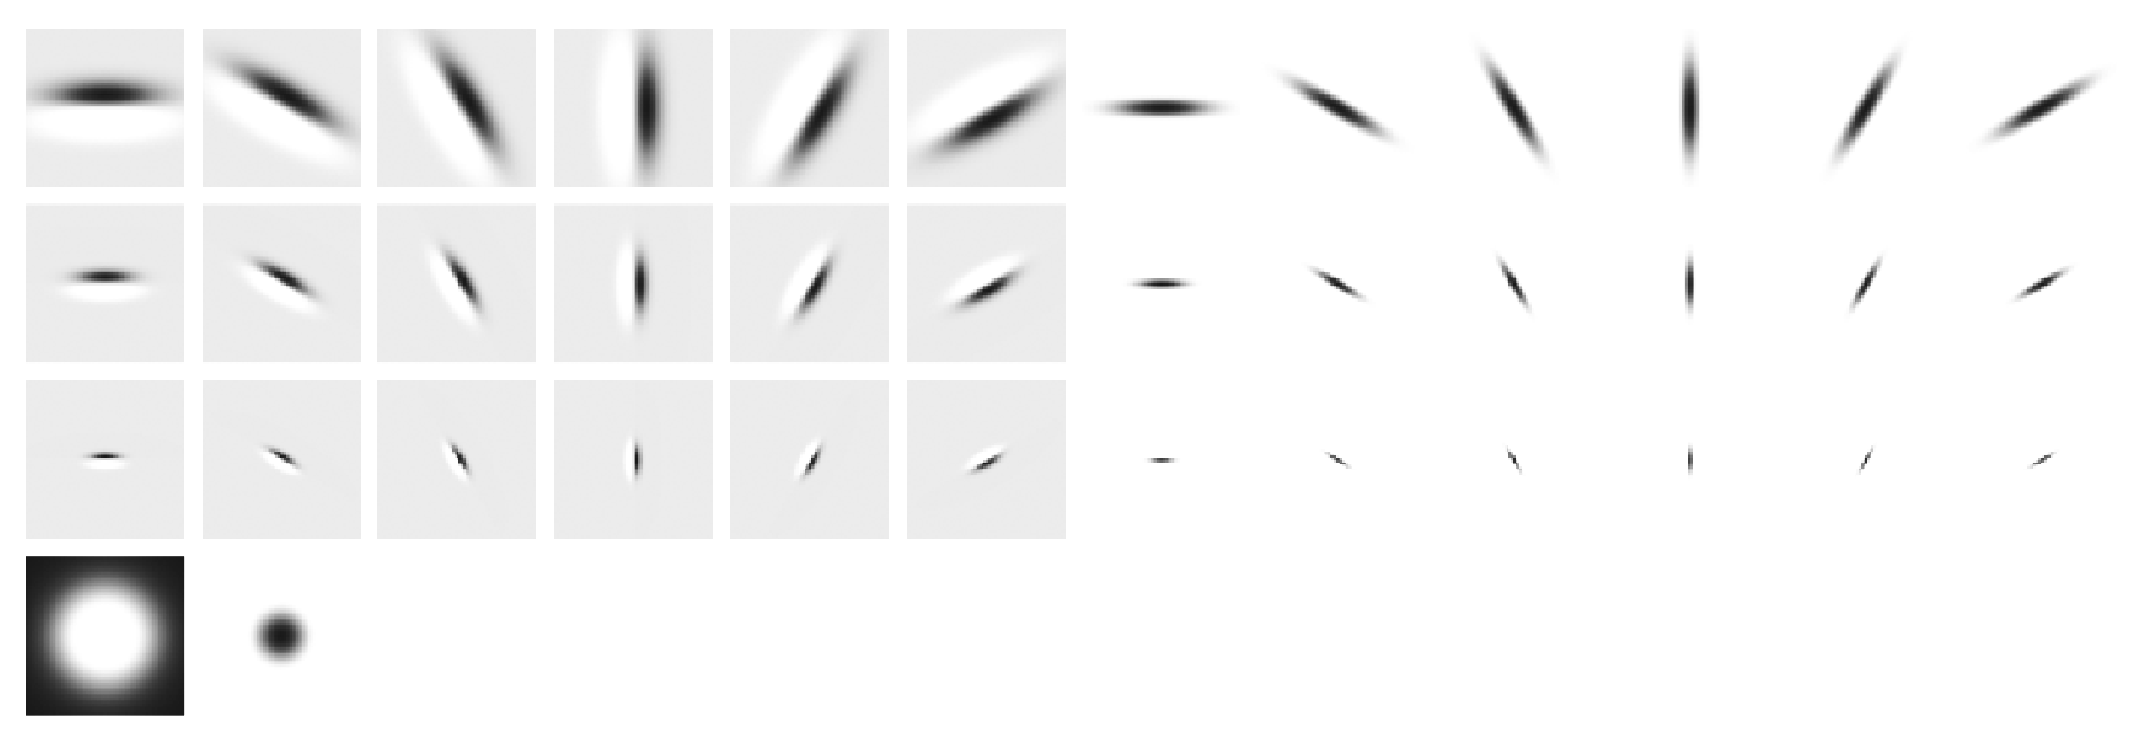
\epsfig{file=images/MR.eps, width=0.6\linewidth}
	\end{center}
	\caption{\textit{The Maximum Response filter bank consisting of 2 anisotropic edge and bar filters at 6 orientations and 3 scales and 2 isotropic filters, a Gaussian and Laplacian of Gaussian. A total of 38 filters, but only 6 filter responses of the anisotropic filters across orientations and the 2 responses of the isotropic filters are registered.}}
	\label{fig:MR}
\end{figure}

\section{Multivariate Gaussian Distributions}\label{sec:MGD}
A drawback of the texton approach is the need for a texton dictionary, which requires clustering in high-dimensional spaces. This poses problems when the number of classes and image data increase as it becomes intractable to compute the clusters. At the same time, the idea of using textons implies that more data is needed to capture general properties that characterizes the data correctly.

Broadhurst presents a parametric approach to estimate the likelihood of homogeneously textured images \cite{Broadhurst}. His work extends the framework proposed by Levina \cite{Levina} by using a Gaussian Bayes classifier instead of a Nearest Neighbor classifier. To model each material class, Broadhurst uses multivariate Gaussian distributions to model the intra-class variability of the marginals within a material class. This is done by constructing marginal histograms out of filter responses, then mapping the joint of the marginal histograms into Euclidean space and applying principal component analysis (PCA) to obtain eigencomponents for each class. With this approach, there is no need for a texton dictionary. The use of a dictionary limits the generalization of a texture class and also needs clustering in high-dimensional spaces, making the problem intractable when extending the number of classes. 

\todo{Although less descriptive than joint conditional distributions, the dependencies among filter responses are captured by estimating the joint intra-class variation of the marginal histograms. This approach increases the descriptive power of the marginal distributions while still maintaining the computational efficiency.}

In order to perform statistical analysis on the marginal distributions, the distributions are mapped to points in Euclidean space. Responses are represented as marginal histograms by sorting the response values in descending order and store the average response value of each bin, creating so-called eqi-count histograms. To compare these discrete distributions, consider two equi-count histograms $x$ and $y$ with $n$ bins and the average value of each bin stored, with their values sorted in descending order. The distributions $x$ and $y$ are represented as vectors of $n$ bin values. The Mallow Distance is used to measure distribution similarity in the Euclidean space. The Mallows distance between these vectors is given by:

	\begin{eqnarray*}
		M_2(x, y) = (\sum^n_{i=1} ||x_i - y_i||)^{1/2}
	\end{eqnarray*}

The described representation maps histograms to points in Euclidean space with distances corresponding to $M_2$ histogram distances. Experiments are run on samples from the {\it CUReT} database, which consists of 61 texture classes with each 205 different viewing and illumination conditions. Each class experiences $3\mathcal{D}$ effect such as interreflections, speculars and shadowing, which gives a large intra-class variability. In a preprocessing step, the images are converted to gray-scale and are processed to have zero-mean and unit-variance to have intensity invariance. The MR8 filter bank is used to gain rotationally invariant features by using the maximum responses over the orientations as done in the works described in \ref{sec:Textons}.

%Levinka has developed a framework for classification using filter banks, marginal histograms, the Mallow distance and a 1NN classifier. The 1-NN classifier requires a distance measure between two sets of marginal distributions. Broadhurst defines this to be the product of the M2 marginal distances described in section 2. The variation of marginal distributions can be measured jointly or independently. A joint 1-NN classifier measures the distance between a target image and all the training images as the distance between each set of marginals. The target image is then classified using the closest training image. For an independent 1-NN classifier, the minimum M2 distance between each target marginal and each class is computed. The total distance to a class is defined as the product of each minimum marginal distance.

In his experiments, Broadhurst considers both independent marginal and joint marginal variation for construction of the Gaussian models. To construct models based on independent marginal variation, eqi-count histograms for each image their 8 maximum responses are computed. The number of histograms chosen in his experiments are 10, 25, 100 and a 1000 bins. PCA is applied to obtain 8 feature specific subspaces per material class, a subspace for each of the filter responses over all training images. For classification, a novel image is projected on the subspaces of each material class and the projection error is computed. The class with the lowest projection error is considered the class of the novel image.

In the experiments conducted by Broadhurst, the joint marginal based models performed significantly better than the independent marginal based models, with $\pm 95\%$ for independent marginals and $\pm 99\%$ for joint marginals. The best performance was measured on histograms with 25 bins.


%After the histograms are computed, PCA is applied to estimate the Gaussian distribution in a lower dimensional subspace for each class and marginal. The number of eigencomponents used differs for the number of bins in the histogram representation, 6, 7, 8 and 9 respectively. As a result, a class is represented by 8 Gaussian models with dimensions equal to the respective number of eigencomponents. 

%For the models based on joint marginal variation, the computed marginals for each image are concatenated into 1 long vector. For each class, PCA is applied on these long vectors to estimate the Gaussian distribution in low dimensional subspace. This gives 1 Gaussian model for each class. To classify novel images, the test image is assigned to the class with the maximum likelihood containing that image. Because all priors are equal for each class, this translates into a Bayes classification problem.


\section{Minimal Training Images}\label{sec:Minimal}

For the construction of models in both methods described in section \ref{sec:Textons} and \ref{sec:MGD}, a lot of image data is required to capture the intra-class variation of the material. This seriously limits the computed descriptors to the amount of illumination and view conditions available in the training data, thus incapable of generalizing effectively beyond the presented data.

In his research, Targhi's central goal is to reduce the amount of images needed for training and yet still produce the same (or better) classification results \cite{Targhi}. With proper reconstruction of surface albedo and surface normals of a material, its possible to generate novel image data with arbitrary viewing and illumination conditions. Using a simple model of photometric stereo, only a small set of original image data is needed for the synthesis of new image data.

For the synthesis of new image data, the Lambertian reflectance model is used. This method effectively simulates diffuse reflection from materials as well as self-shadows, but not more complex light phenomena such as speculars or interreflections. 

Experiments are run on two material databases which are designed for the purpose of physical based texture classification; \textit{ALOT} (\textit{Amsterdam Library of Textures}) and \textit{PhoTex}, a library of photometric image data for texture recognition. The training and testing of the classifier is done by replicating the experiments of Broadhurst. Details on Photex will be outlined in section \ref{sec:PhoTex}. The experimental setup will be described in more detail in section \ref{sec:Experiments}.

Targhi reported improvement over the state-of-the-art results of classification on both databases by augmenting the training data with synthesized data using a minimal amount of images needed for photometric stereo. However, using only the Lambertian reflectance model for image synthesis, it is expected that its application is constrained to diffuse materials. For the synthesis of non-diffuse or non-Lambertian image data, other reflection models are required. More sophisticated reflection models could enhance the quality of the synthetic image data and make it possible to incorporate certain illumination phenomena such as speculars, interreflections and backscattering. 


	\chapter{Approach}
	\hypertarget{Approach}{
\section{Photometric Stereo}\label{PhotometricStereo}
}

\begin{itemize}
	\item{core formula}
	\item{Lambertian assumption}
\end{itemize}

\section{Reflection Models}
\begin{itemize}
	\item{Lambertian}
	\item{Phong, Blinn-Phong}
	\item{Ward}
	\item{Lafortune}
	\item{Microfacets}
	\item{Cook-Torrance}
	\item{Oren-Nayar}
\end{itemize}



\section{Classification}
\begin{itemize}
	\item{multivariate Gaussian Classifier, Mallow distance}
	\item{Texton Dictionary, Chi-distance}
\end{itemize}


	%___________________________________________________________________________________________
 	\nocite{*}
	\bibliographystyle{plain}
	\bibliography{bibtex}
	\printindex
\end{document}

